\documentclass[12pt,a4paper]{article}

\newcommand{\TETELNUMBER}{13}
\newcommand{\TETELTITLE}{Java alapok, objektumok, szemétgyűjtés és kivételkezelés}
\newcommand{\TETELSHORTTITLE}{Java és OOP alapok}

\newcommand{\ZVTetelsorDataOnly}{}
\newcommand{\ZVTetelOne}{Adatok, adattípusok, adatműveletek és adatstruktúrák. Szám adattípus. Számrendszerek, konverziók. A logikai, halmaz, karakter, sztring absztrakt adattípusok és realizációjuk. A tömb (vektor, mátrix), rekord absztrakt adattípusok.}
\newcommand{\ZVTetelTwo}{Az algoritmus. Iteratív és rekurzív algoritmus. A számítógépes memória. Adat és program. Verem és procedúra. Az algoritmus lejegyzése. A folyamatábra és a pszeudokód. Elemi algoritmusok.}
\newcommand{\ZVTetelThree}{Strukturált programozás. Programgráf, valódi program, vezérlőgráf lebontása, strukturált program és annak formulája. Strukturált programgráf kialakítása, struktogram. Ciklikus bonyolultság és egyéb bonyolultsági tételek.}
\newcommand{\ZVTetelFour}{Számelméleti algoritmusok. Legnagyobb közös osztó, euklideszi és kibővített euklideszi algoritmus, lineáris kongruencia egyenletek. Multiplikatív inverz, moduláris hatványozás, Fermat prímteszt. RSA.}
\newcommand{\ZVTetelFive}{Rendezések: Beszúró rendezés. Az ,,Oszd meg és uralkodj!'' elv. Összefésülő rendezés. Gyors rendezés. Buborék rendezés. Shell rendezés. Minimum kiválasztásos rendezés. Négyzetes rendezés. Lineáris idejű rendezések: leszámláló rendezés, számjegyes rendezés. Időelemzéseik. Az összehasonlító rendezések időtétele.}
\newcommand{\ZVTetelSix}{Gráfalgoritmusok. Szélességi keresés. Mélységi keresés. Topologikus rendezés. Optimumfeladatok fákon (minimális feszítőfák, Kruskal- és Prim-algoritmus). Legrövidebb utak meghatározása (Dijkstra-algoritmus, Bellman--Ford-algoritmus, Floyd--Warshall-algoritmus).}
\newcommand{\ZVTetelSeven}{A párhuzamos algoritmusok alapfogalmai, PRAM modell, hatékonysági mértékek (munka, költség, gyorsítás, hatékonyság). Párhuzamos végrehajtás ábrázolási módjai. Komplexitás becslése, párhuzamos komplexitás. Amdahl törvénye. Pipeline párhuzamosítás, Lost update probléma bemutatása és megoldása.}
\newcommand{\ZVTetelEight}{Aggregáció, redukció, prefixszámítás párhuzamosítási lehetőségei. \texttt{CREW\_PREFIX}, \texttt{EREW\_PREFIX} és \texttt{OPTIMAL\_PREFIX} algoritmusok bemutatása. Összefésülő rendezés párhuzamosítási módja.}
\newcommand{\ZVTetelNine}{A busz, gyűrű, rács, tórusz, hiperkocka és fa topológiák bemutatása, csomópontok közötti távolságok jellemzése. A CSP, Publish--Subscribe és az Aktor modell. Az aszinkron programozás elemei: async, await kulcsszavak használata, coroutine-ok.}
\newcommand{\ZVTetelTen}{A Turing-gép fogalma, működése. A RAM-gép. Boole-függvények és logikai hálózatok.}
\newcommand{\ZVTetelEleven}{Algoritmikus eldönthetőség. Church-tézis. Rekurzív és rekurzívan felsorolható nyelvek, rekurzív illetve parciálisan rekurzív függvények. Nevezetes nyelvek (Az R, Re, coR, coRE nyelvosztályok és ezek kapcsolata) és bonyolultságuk. Algoritmikusan eldönthetetlen problémák. Polinomiális idejű algoritmusok.}
\newcommand{\ZVTetelTwelve}{Nemdeterminisztikus Turing-gépek, az NP és a coNP nyelvosztály. Példák NP-beli nyelvekre. A tanú-tétel. Nemdeterminisztikus algoritmusok bonyolultsága. NP-teljesség, Cook-tétel. Néhány NP-teljes probléma, Cook--Levin-tétel.}
\newcommand{\ZVTetelThirteen}{A Java programozási nyelv története, alapvető jellemzői. Egy Java program szerkezete (csomagok és fordítási egységek). Az objektumorientált programtervezés alapelveinek felsorolása. Objektumok tárolása és élettartama. Szemétgyűjtő mechanizmus. Kivételkezelés.}
\newcommand{\ZVTetelFourteen}{Az egységbezárás és az információrejtés objektumorientált alapelvek megvalósítása. Osztálydefiníció és példányosítás. Osztályszintű és példányszintű tagok, konstansok. Hozzáférési kategóriák és használatuk. Hivatkozás az osztály tagjaira.}
\newcommand{\ZVTetelFifteen}{Az öröklődés és a polimorfizmus objektumorientált alapelvek megvalósítása. Öröklődés szabályai, metódusok túlterhelése és felüldefiniálása. A referencia statikus és dinamikus típusa. Absztrakt osztály és interfész szerepe, összehasonlítása.}
\newcommand{\ZVTetelSixteen}{Az operációs rendszerbeli folyamat (processz) fogalma. Folyamatkontextus. A fonál (szál) fogalma. A processzállapotok, állapotváltások, processz futási módok. Taszk- és fonálállapotok, állapotátmenetek.}
\newcommand{\ZVTetelSeventeen}{A memóriamenedzselés feladatai. Memória mint erőforrás. Címleképzés fajtái. Lapozós virtuális memóriamenedzselés működése. Allokálás, nyilvántartás, címleképzés. Laphiba fogalma, kezelése, kilapozási stratégiák. Előnyök, hátrányok.}
\newcommand{\ZVTetelEighteen}{Fájlrendszer-megvalósítási feladatok. Jegyzékszerkezetek. Szabadblokk-menedzselési lehetőségek. Fájlattribútum-rögzítési lehetőségek (ezen belül a fájltestet képező blokkok rögzítési lehetőségei).}
\newcommand{\ZVTetelNineteen}{Relációs adatmodell, relációs struktúra és integritási feltételek. ER modell elemei jelentése és jelölése. Az ER modell konverziója relációs modellre. Relációs adatmodell műveleti része, relációs algebra.}
\newcommand{\ZVTetelTwenty}{Az SQL szabvány relációs adatbázis kezelő nyelv bemutatása, a DDL (objektum létrehozás, megszüntetés és szerkezet módosítás), DML (rekord felvitel, törlés és módosítás), DCL és a SELECT utasítások áttekintése és használata. Beágyazott SELECT használata. A relációs algebra műveleteinek megvalósítása SQL-ben.}
\newcommand{\ZVTetelTwentyOne}{Adatkezelés és adatbáziskezelés alapfogalmai, fileszervezési módszerek, B-fa index; adatbázis architektúra; A normalizálás szerepe a relációs adatbázis kezelésben. Redundancia oka és a megszüntetés lépései. Normálformák. Dekompozíció célja és szabályai, tételei.}
\newcommand{\ZVTetelTwentyTwo}{Számítógép-hálózatokhoz kötődő alapfogalmak és az ISO--OSI hivatkozási modell: topológia és méret szerinti osztályozásuk. Kapcsolástechnika szerinti osztályozásuk (vonalkapcsolás, üzenetkapcsolás, csomagkapcsolás és virtuális vonalkapcsolás). Az ISO--OSI hivatkozási modell szerkezete, rétegei és azok főbb funkciói.}
\newcommand{\ZVTetelTwentyThree}{A számítógép-hálózatok ISO--OSI hivatkozási modell adatkapcsolati rétegének közeghozzáférési alrétege: A főbb csatorna-megosztási osztályok (statikus-dinamikus, dinamikus versengő-determinisztikus) bemutatása és azok összevetése. Az IEEE 802.3 és az Ethernet (CSMA/CD) keretformátum, MAC címek, támogatott közegek és sebességek bemutatása, működés duplex csatorna esetén. Az IEEE 802.11 WLAN általános felépítése, az Access Point (AP) főbb funkciói. Az alkalmazott közeghozzáférési módszer (CSMA/CA), Distributed Coordination Function (DCF) és Point Coordination Function (PCF) üzemmódok.}
\newcommand{\ZVTetelTwentyFour}{A TCP/IP protokollszövet és az Internet. Az Internet hivatkozási modell (DoD) és az ISO--OSI hivatkozási modell összevetése. A TCP/IP protokollszövet főbb részei (ARP, RARP, IP, ICMP, TCP, UDP) és azok funkciói. Az internetes címzés és címosztályok: IPv4-címosztályok, maszk, subnet, supernet, osztály nélküli címzés (CIDR -- Classless Inter-Domain Routing) és változó alhálózat-méretek (VLSM -- Variable Length Subnet Mask), címek kiosztása, lokális címek és címfordítás (NAT). IPv6-címek, IPv6-címtípusok (unicast, multicast, anycast; link local, unique local, aggregatable global unicast address).}
\newcommand{\ZVTetelTwentyFive}{Szoftvertechnológia és a szoftverfolyamat fogalma. A szoftverfolyamat-fázisok részletes bemutatása: szoftverspecifikáció, tervezés, implementáció, validáció és evolúció. Az evolúciós modell ismertetése.}
\newcommand{\ZVTetelTwentySix}{Szoftverkövetelmény fogalma és osztályozásai. Követelmények általános problémái. Követelményfeltárás és -elemzés folyamata. Vezérlési stílusok.}
\newcommand{\ZVTetelTwentySeven}{UML diagramok bemutatása: Use case és osztálydiagram. A szekvenciadiagram. Komponensdiagram.}

\newcommand{\ZVTetelKiiras}[1]{%
  \ifcase#1\relax
  \or \ZVTetelOne
  \or \ZVTetelTwo
  \or \ZVTetelThree
  \or \ZVTetelFour
  \or \ZVTetelFive
  \or \ZVTetelSix
  \or \ZVTetelSeven
  \or \ZVTetelEight
  \or \ZVTetelNine
  \or \ZVTetelTen
  \or \ZVTetelEleven
  \or \ZVTetelTwelve
  \or \ZVTetelThirteen
  \or \ZVTetelFourteen
  \or \ZVTetelFifteen
  \or \ZVTetelSixteen
  \or \ZVTetelSeventeen
  \or \ZVTetelEighteen
  \or \ZVTetelNineteen
  \or \ZVTetelTwenty
  \or \ZVTetelTwentyOne
  \or \ZVTetelTwentyTwo
  \or \ZVTetelTwentyThree
  \or \ZVTetelTwentyFour
  \or \ZVTetelTwentyFive
  \or \ZVTetelTwentySix
  \or \ZVTetelTwentySeven
  \fi
}

\newcommand{\ZVTetelsorList}{%
\begin{enumerate}[leftmargin=7mm,label=\arabic*.,itemsep=2pt,topsep=2pt,parsep=0pt]
  \item \ZVTetelOne
  \item \ZVTetelTwo
  \item \ZVTetelThree
  \item \ZVTetelFour
  \item \ZVTetelFive
  \item \ZVTetelSix
  \item \ZVTetelSeven
  \item \ZVTetelEight
  \item \ZVTetelNine
  \item \ZVTetelTen
  \item \ZVTetelEleven
  \item \ZVTetelTwelve
  \item \ZVTetelThirteen
  \item \ZVTetelFourteen
  \item \ZVTetelFifteen
  \item \ZVTetelSixteen
  \item \ZVTetelSeventeen
  \item \ZVTetelEighteen
  \item \ZVTetelNineteen
  \item \ZVTetelTwenty
  \item \ZVTetelTwentyOne
  \item \ZVTetelTwentyTwo
  \item \ZVTetelTwentyThree
  \item \ZVTetelTwentyFour
  \item \ZVTetelTwentyFive
  \item \ZVTetelTwentySix
  \item \ZVTetelTwentySeven
\end{enumerate}%
}


\newcommand{\tetelsorrow}[2]{\textbf{#1.} & #2\tabularnewline}

\newcommand{\tetelsorpageone}{%
\begin{tabularx}{\textwidth}{|>{\raggedleft\bfseries}p{8mm}@{\hspace{5mm}}>{\raggedright\arraybackslash}X|}
\hline
\tetelsorrow{1}{\ZVTetelOne}
\tetelsorrow{2}{\ZVTetelTwo}
\tetelsorrow{3}{\ZVTetelThree}
\hline
\tetelsorrow{4}{\ZVTetelFour}
\tetelsorrow{5}{\ZVTetelFive}
\tetelsorrow{6}{\ZVTetelSix}
\hline
\tetelsorrow{7}{\ZVTetelSeven}
\tetelsorrow{8}{\ZVTetelEight}
\tetelsorrow{9}{\ZVTetelNine}
\hline
\tetelsorrow{10}{\ZVTetelTen}
\tetelsorrow{11}{\ZVTetelEleven}
\tetelsorrow{12}{\ZVTetelTwelve}
\hline
\end{tabularx}%
}

\newcommand{\tetelsorpagetwo}{%
\begin{tabularx}{\textwidth}{|>{\raggedleft\bfseries}p{8mm}@{\hspace{5mm}}>{\raggedright\arraybackslash}X|}
\hline
\tetelsorrow{13}{\ZVTetelThirteen}
\tetelsorrow{14}{\ZVTetelFourteen}
\tetelsorrow{15}{\ZVTetelFifteen}
\hline
\tetelsorrow{16}{\ZVTetelSixteen}
\tetelsorrow{17}{\ZVTetelSeventeen}
\tetelsorrow{18}{\ZVTetelEighteen}
\hline
\tetelsorrow{19}{\ZVTetelNineteen}
\tetelsorrow{20}{\ZVTetelTwenty}
\tetelsorrow{21}{\ZVTetelTwentyOne}
\hline
\tetelsorrow{22}{\ZVTetelTwentyTwo}
\tetelsorrow{23}{\ZVTetelTwentyThree}
\tetelsorrow{24}{\ZVTetelTwentyFour}
\hline
\tetelsorrow{25}{\ZVTetelTwentyFive}
\tetelsorrow{26}{\ZVTetelTwentySix}
\tetelsorrow{27}{\ZVTetelTwentySeven}
\hline
\end{tabularx}%
}

\ifdefined\ZVTetelsorDataOnly
\expandafter\endinput
\fi

\documentclass[10pt,a4paper]{article}
\newcommand{\ZVHEADERLEFT}{Záróvizsga tételek}
\newcommand{\ZVHEADERRIGHT}{Programtervező informatikus BSc}
\usepackage{fontspec}
\usepackage{geometry}
\usepackage{microtype}
\usepackage{xcolor}
\usepackage{amsmath,amssymb,mathtools}
\usepackage{booktabs,longtable,tabularx,array,multirow}
\usepackage{enumitem}
\usepackage{hyperref}
\usepackage{fancyhdr}
\usepackage{titlesec}
\usepackage{listings}
\usepackage[most]{tcolorbox}
\usepackage{tikz}
\usetikzlibrary{positioning,shapes.geometric,shapes.misc,arrows.meta,decorations.pathreplacing}
\usepackage{caption}

\setlength{\headheight}{16pt}
\emergencystretch=2em
\renewcommand{\contentsname}{Tartalom}

% Fontbeallitasok: ha a DejaVu fontok nincsenek telepitve,
% akkor automatikusan a MiKTeX/TeX Live alap Latin Modern fontjaira valtunk.
\IfFontExistsTF{DejaVu Serif}{\setmainfont{DejaVu Serif}}{\setmainfont{Latin Modern Roman}}
\IfFontExistsTF{DejaVu Sans}{\setsansfont{DejaVu Sans}}{\setsansfont{Latin Modern Sans}}
\IfFontExistsTF{DejaVu Sans Mono}{\setmonofont{DejaVu Sans Mono}}{\setmonofont{Latin Modern Mono}}

\geometry{left=25mm,right=25mm,top=24mm,bottom=27mm}

\hypersetup{
  colorlinks=true,
  linkcolor=blue!45!black,
  urlcolor=blue!55!black,
  pdftitle={Zarovizsga tetel},
  pdfauthor={Baba Levente - tanulasi segedanyag}
}

\definecolor{accent}{HTML}{1F4E79}
\definecolor{lightaccent}{HTML}{EAF2F8}
\definecolor{warnbg}{HTML}{FFF4E5}
\definecolor{codebg}{HTML}{F7F7F7}

\tikzset{
  flow/.style={draw, rounded corners, align=center, minimum width=21mm, minimum height=8mm, fill=lightaccent},
  pred/.style={draw, diamond, aspect=2, align=center, inner sep=1pt, fill=warnbg},
  merge/.style={draw, circle, inner sep=1.2pt, fill=black!8},
  terminator/.style={draw, rounded corners=4mm, align=center, minimum width=20mm, minimum height=8mm, fill=black!5},
  arrow/.style={->, >=stealth, thick},
  zvflowstart/.style={draw, rounded rectangle, minimum width=2.3cm, minimum height=0.7cm, align=center},
  zvflowprocess/.style={draw, rectangle, minimum width=2.7cm, minimum height=0.7cm, align=center},
  zvflowdecision/.style={draw, diamond, aspect=2.2, minimum width=2.8cm, minimum height=0.8cm, align=center}
}


\titleformat{\section}{\Large\bfseries\sffamily\color{accent}}{\thesection.}{0.6em}{}
\titleformat{\subsection}{\large\bfseries\sffamily\color{accent}}{\thesubsection.}{0.6em}{}
\titleformat{\subsubsection}{\normalsize\bfseries\sffamily\color{accent}}{\thesubsubsection.}{0.6em}{}

\setlist[itemize]{topsep=3pt,itemsep=2pt,parsep=0pt,leftmargin=1.4em}
\setlist[enumerate]{topsep=3pt,itemsep=2pt,parsep=0pt,leftmargin=1.6em}
\setlength{\parindent}{0pt}
\setlength{\parskip}{6pt}
\renewcommand{\arraystretch}{1.25}
\newcolumntype{L}[1]{>{\raggedright\arraybackslash}p{#1}}
\renewcommand{\tabularxcolumn}[1]{>{\raggedright\arraybackslash}p{#1}}

\providecommand{\ZVHEADERLEFT}{\TETELNUMBER. tétel}
\providecommand{\ZVHEADERRIGHT}{\TETELSHORTTITLE}

\pagestyle{fancy}
\fancyhf{}
\lhead{\ZVHEADERLEFT}
\rhead{\ZVHEADERRIGHT}
\cfoot{\thepage}

\lstdefinelanguage{pseudocode}{
  morekeywords={IF,THEN,ELSE,WHILE,DO,FOR,TO,DOWNTO,REPEAT,UNTIL,RETURN,CALL,INPUT,OUTPUT,AND,OR,NOT,TRUE,FALSE},
  sensitive=true,
  morecomment=[l]{//}
}

\lstdefinestyle{code}{
  basicstyle=\ttfamily\small,
  backgroundcolor=\color{codebg},
  frame=single,
  rulecolor=\color{black!15},
  columns=fullflexible,
  keepspaces=true,
  breaklines=true,
  tabsize=2,
  showstringspaces=false,
  numbers=left,
  numberstyle=\tiny\color{black!55},
  numbersep=7pt,
  xleftmargin=2.2em,
  framexleftmargin=1.7em,
  captionpos=b
}

\lstdefinestyle{pseudo}{
  style=code,
  language=pseudocode,
  keywordstyle=\bfseries\color{accent!85!black},
  commentstyle=\itshape\color{black!55}
}

\lstdefinestyle{csource}{
  style=code,
  language=C,
  keywordstyle=\bfseries\color{accent!85!black},
  commentstyle=\itshape\color{black!55},
  stringstyle=\color{orange!70!black}
}

\lstset{style=code}
\renewcommand{\lstlistingname}{Kódrészlet}
\renewcommand{\lstlistlistingname}{Kódrészletek}
\newcommand{\zvcode}[2][]{\lstinputlisting[style=code,#1]{#2}}
\newcommand{\zvpseudocode}[2][]{\lstinputlisting[style=pseudo,#1]{#2}}
\newcommand{\zvccode}[2][]{\lstinputlisting[style=csource,#1]{#2}}

\newtcolorbox{summarybox}{
  enhanced,
  colback=lightaccent,
  colframe=accent!70!black,
  arc=2mm,
  boxrule=0.5pt,
  left=2mm,right=2mm,top=1mm,bottom=1mm
}

\newtcolorbox{warningbox}{
  enhanced,
  colback=warnbg,
  colframe=orange!70!black,
  arc=2mm,
  boxrule=0.5pt,
  left=2mm,right=2mm,top=1mm,bottom=1mm
}

\newcommand{\adt}[2]{\ensuremath{#1=(#2)}}
\newcommand{\set}[1]{\ensuremath{\{#1\}}}
\newcommand{\code}[1]{\texttt{#1}}
\newcommand{\base}[2]{\ensuremath{#1_{(#2)}}}
\newcommand{\addr}{\ensuremath{@}}


\providecommand{\TETELKIIRAS}{\TETELTITLE. \TETELTOPIC}
\providecommand{\ZVAUTHOR}{Baba Levente}
\providecommand{\ZVYEAR}{2026}
\providecommand{\ZVAID}{ChatGPT segítségével}

\newcommand{\makezvtitle}{%
\begin{titlepage}
  \centering
  \vspace*{18mm}
  {\Large\sffamily Programtervező Informatikus BSc\par}
  \vspace{1mm}
  {\large\sffamily \ZVYEAR-os záróvizsga tételek\par}
  \vspace{15mm}
  {\Huge\bfseries\sffamily \TETELNUMBER. tétel\par}
  \vspace{5mm}
  {\LARGE\bfseries\sffamily \TETELTITLE\par}
  \vspace{10mm}
  \begin{summarybox}
    \textbf{Tételkiírás:} \TETELKIIRAS
  \end{summarybox}
  \vfill
  {\large Készítette: \textbf{\ZVAUTHOR}\par}
  \vspace{2mm}
  {\large \ZVAID\par}
\end{titlepage}%
}

\newcommand{\zvfrontmatter}{%
  \sloppy
  \makezvtitle
  \tableofcontents
  \newpage
}

\begin{document}
\newgeometry{left=13mm,right=13mm,top=13mm,bottom=13mm}
\pagestyle{empty}
\setlength{\tabcolsep}{2.6pt}
\renewcommand{\arraystretch}{1.08}
\begin{center}
  {\Huge\bfseries Záróvizsga tételek\par}
  \vspace{2mm}
  {\Large\itshape Programtervező informatikus BSc\par}
\end{center}
\vspace{10mm}
{\fontsize{10.5}{12.2}\selectfont
\tetelsorpageone
}
\newpage
{\fontsize{10.5}{12.2}\selectfont
\tetelsorpagetwo
}
\end{document}

\newcommand{\TETELKIIRAS}{\ZVTetelKiiras{\TETELNUMBER}}

\usepackage{fontspec}
\usepackage{geometry}
\usepackage{microtype}
\usepackage{xcolor}
\usepackage{amsmath,amssymb,mathtools}
\usepackage{booktabs,longtable,tabularx,array,multirow}
\usepackage{enumitem}
\usepackage{hyperref}
\usepackage{fancyhdr}
\usepackage{titlesec}
\usepackage{listings}
\usepackage[most]{tcolorbox}
\usepackage{tikz}
\usetikzlibrary{positioning,shapes.geometric,shapes.misc,arrows.meta,decorations.pathreplacing}
\usepackage{caption}

\setlength{\headheight}{16pt}
\emergencystretch=2em
\renewcommand{\contentsname}{Tartalom}

% Fontbeallitasok: ha a DejaVu fontok nincsenek telepitve,
% akkor automatikusan a MiKTeX/TeX Live alap Latin Modern fontjaira valtunk.
\IfFontExistsTF{DejaVu Serif}{\setmainfont{DejaVu Serif}}{\setmainfont{Latin Modern Roman}}
\IfFontExistsTF{DejaVu Sans}{\setsansfont{DejaVu Sans}}{\setsansfont{Latin Modern Sans}}
\IfFontExistsTF{DejaVu Sans Mono}{\setmonofont{DejaVu Sans Mono}}{\setmonofont{Latin Modern Mono}}

\geometry{left=25mm,right=25mm,top=24mm,bottom=27mm}

\hypersetup{
  colorlinks=true,
  linkcolor=blue!45!black,
  urlcolor=blue!55!black,
  pdftitle={Zarovizsga tetel},
  pdfauthor={Baba Levente - tanulasi segedanyag}
}

\definecolor{accent}{HTML}{1F4E79}
\definecolor{lightaccent}{HTML}{EAF2F8}
\definecolor{warnbg}{HTML}{FFF4E5}
\definecolor{codebg}{HTML}{F7F7F7}

\tikzset{
  flow/.style={draw, rounded corners, align=center, minimum width=21mm, minimum height=8mm, fill=lightaccent},
  pred/.style={draw, diamond, aspect=2, align=center, inner sep=1pt, fill=warnbg},
  merge/.style={draw, circle, inner sep=1.2pt, fill=black!8},
  terminator/.style={draw, rounded corners=4mm, align=center, minimum width=20mm, minimum height=8mm, fill=black!5},
  arrow/.style={->, >=stealth, thick},
  zvflowstart/.style={draw, rounded rectangle, minimum width=2.3cm, minimum height=0.7cm, align=center},
  zvflowprocess/.style={draw, rectangle, minimum width=2.7cm, minimum height=0.7cm, align=center},
  zvflowdecision/.style={draw, diamond, aspect=2.2, minimum width=2.8cm, minimum height=0.8cm, align=center}
}


\titleformat{\section}{\Large\bfseries\sffamily\color{accent}}{\thesection.}{0.6em}{}
\titleformat{\subsection}{\large\bfseries\sffamily\color{accent}}{\thesubsection.}{0.6em}{}
\titleformat{\subsubsection}{\normalsize\bfseries\sffamily\color{accent}}{\thesubsubsection.}{0.6em}{}

\setlist[itemize]{topsep=3pt,itemsep=2pt,parsep=0pt,leftmargin=1.4em}
\setlist[enumerate]{topsep=3pt,itemsep=2pt,parsep=0pt,leftmargin=1.6em}
\setlength{\parindent}{0pt}
\setlength{\parskip}{6pt}
\renewcommand{\arraystretch}{1.25}
\newcolumntype{L}[1]{>{\raggedright\arraybackslash}p{#1}}
\renewcommand{\tabularxcolumn}[1]{>{\raggedright\arraybackslash}p{#1}}

\providecommand{\ZVHEADERLEFT}{\TETELNUMBER. tétel}
\providecommand{\ZVHEADERRIGHT}{\TETELSHORTTITLE}

\pagestyle{fancy}
\fancyhf{}
\lhead{\ZVHEADERLEFT}
\rhead{\ZVHEADERRIGHT}
\cfoot{\thepage}

\lstdefinelanguage{pseudocode}{
  morekeywords={IF,THEN,ELSE,WHILE,DO,FOR,TO,DOWNTO,REPEAT,UNTIL,RETURN,CALL,INPUT,OUTPUT,AND,OR,NOT,TRUE,FALSE},
  sensitive=true,
  morecomment=[l]{//}
}

\lstdefinestyle{code}{
  basicstyle=\ttfamily\small,
  backgroundcolor=\color{codebg},
  frame=single,
  rulecolor=\color{black!15},
  columns=fullflexible,
  keepspaces=true,
  breaklines=true,
  tabsize=2,
  showstringspaces=false,
  numbers=left,
  numberstyle=\tiny\color{black!55},
  numbersep=7pt,
  xleftmargin=2.2em,
  framexleftmargin=1.7em,
  captionpos=b
}

\lstdefinestyle{pseudo}{
  style=code,
  language=pseudocode,
  keywordstyle=\bfseries\color{accent!85!black},
  commentstyle=\itshape\color{black!55}
}

\lstdefinestyle{csource}{
  style=code,
  language=C,
  keywordstyle=\bfseries\color{accent!85!black},
  commentstyle=\itshape\color{black!55},
  stringstyle=\color{orange!70!black}
}

\lstset{style=code}
\renewcommand{\lstlistingname}{Kódrészlet}
\renewcommand{\lstlistlistingname}{Kódrészletek}
\newcommand{\zvcode}[2][]{\lstinputlisting[style=code,#1]{#2}}
\newcommand{\zvpseudocode}[2][]{\lstinputlisting[style=pseudo,#1]{#2}}
\newcommand{\zvccode}[2][]{\lstinputlisting[style=csource,#1]{#2}}

\newtcolorbox{summarybox}{
  enhanced,
  colback=lightaccent,
  colframe=accent!70!black,
  arc=2mm,
  boxrule=0.5pt,
  left=2mm,right=2mm,top=1mm,bottom=1mm
}

\newtcolorbox{warningbox}{
  enhanced,
  colback=warnbg,
  colframe=orange!70!black,
  arc=2mm,
  boxrule=0.5pt,
  left=2mm,right=2mm,top=1mm,bottom=1mm
}

\newcommand{\adt}[2]{\ensuremath{#1=(#2)}}
\newcommand{\set}[1]{\ensuremath{\{#1\}}}
\newcommand{\code}[1]{\texttt{#1}}
\newcommand{\base}[2]{\ensuremath{#1_{(#2)}}}
\newcommand{\addr}{\ensuremath{@}}


\providecommand{\TETELKIIRAS}{\TETELTITLE. \TETELTOPIC}
\providecommand{\ZVAUTHOR}{Baba Levente}
\providecommand{\ZVYEAR}{2026}
\providecommand{\ZVAID}{ChatGPT segítségével}

\newcommand{\makezvtitle}{%
\begin{titlepage}
  \centering
  \vspace*{18mm}
  {\Large\sffamily Programtervező Informatikus BSc\par}
  \vspace{1mm}
  {\large\sffamily \ZVYEAR-os záróvizsga tételek\par}
  \vspace{15mm}
  {\Huge\bfseries\sffamily \TETELNUMBER. tétel\par}
  \vspace{5mm}
  {\LARGE\bfseries\sffamily \TETELTITLE\par}
  \vspace{10mm}
  \begin{summarybox}
    \textbf{Tételkiírás:} \TETELKIIRAS
  \end{summarybox}
  \vfill
  {\large Készítette: \textbf{\ZVAUTHOR}\par}
  \vspace{2mm}
  {\large \ZVAID\par}
\end{titlepage}%
}

\newcommand{\zvfrontmatter}{%
  \sloppy
  \makezvtitle
  \tableofcontents
  \newpage
}


\begin{document}
\zvfrontmatter
\section{A tétel lényege és vizsgaszintű vázlata}

\begin{summarybox}
A 13. tétel a Java nyelv és az objektumorientált programozás alapjait kapcsolja össze. A Java lényege, hogy magas szintű, osztályokra épülő, platformfüggetlenségre törekvő nyelv, amely forráskódból bájtkódot készít, ezt pedig a JVM futtatja. A programok fordítási egységekből, csomagokból, osztályokból és metódusokból épülnek fel. Az OOP szemléletben a program együttműködő objektumok rendszere, ahol az objektumok állapotot tárolnak, viselkedést valósítanak meg, életciklusuk pedig a létrehozástól a szemétgyűjtésig tart. A kivételkezelés a rendellenes futási események objektumként való kezelését adja meg.
\end{summarybox}

Vizsgán a tételt célszerű a következő sorrendben felépíteni:

\begin{enumerate}
  \item a Java rövid története és célja: platformfüggetlen, magas szintű, objektumorientált nyelv;
  \item JDK, JRE, JVM, bájtkód, fordítás és futtatás folyamata;
  \item Java program szerkezete: fordítási egység, \code{package}, \code{import}, osztály, \code{main} metódus;
  \item csomagok szerepe: névtér, hozzáférés-szabályozás, teljes név, importálás;
  \item az OOP alapelvei: absztrakció, egységbezárás, információrejtés, öröklés, kompozíció, polimorfizmus;
  \item objektumok tárolása: referencia, stack, heap, statikus adatok;
  \item objektumok élettartama és a szemétgyűjtés elve;
  \item kivételkezelés: \code{try}, \code{catch}, \code{finally}, \code{throw}, \code{throws};
  \item ellenőrzött és nem ellenőrzött kivételek, \code{try-with-resources};
  \item gyakori félreértések és tipikus vizsgaválaszok.
\end{enumerate}

A legfontosabb vizsgamondat: a Java program osztályokból álló, bájtkódra fordított program, amelyet a JVM futtat; objektumai tipikusan a heapen jönnek létre, referenciákon keresztül érhetők el, és a már nem elérhető objektumok memóriáját a szemétgyűjtő szabadítja fel.

\begin{center}
\begin{tabularx}{\textwidth}{L{28mm}L{38mm}X}
\toprule
\textbf{Fogalom} & \textbf{Szerep} & \textbf{Vizsgán fontos megjegyzés} \\
\midrule
Java nyelv & Általános célú, erősen objektumorientált programozási nyelv. & C/C++ jellegű szintaxisra épít, de magasabb szintű: nincs explicit pointeraritmetika, automatikus memóriakezelést használ. \\
JDK & Java Development Kit, fejlesztői csomag. & Tartalmazza többek között a \code{javac} fordítót, a futtatáshoz szükséges eszközöket és a szabványos könyvtárakat. \\
JRE & Java Runtime Environment, futtatókörnyezet. & A lefordított Java program futtatásához szükséges környezet; a fejlesztéshez önmagában nem elég. \\
JVM & Java Virtual Machine, virtuális gép. & A \code{.class} fájlok bájtkódját tölti be, ellenőrzi, értelmezi vagy JIT-fordítja. \\
Bájtkód & Gépfüggetlen köztes kód. & A \code{javac} eredménye nem közvetlen natív gépi kód, hanem JVM által végrehajtható \code{.class} állomány. \\
Platformfüggetlenség & A forrásból fordított bájtkód több rendszeren is futtatható. & A gyakorlati elv: ``write once, run anywhere'', feltéve hogy az adott platformon van megfelelő JVM. \\
Szabványos könyvtár & Kész osztályok és interfészek gyűjteménye. & Ide tartozik például a \code{java.lang}, \code{java.util}, \code{java.io}, \code{java.time}. \\
\bottomrule
\end{tabularx}

\end{center}

\section{A Java nyelv története és alapvető jellemzői}

\subsection{Rövid történeti áttekintés}

A Java fejlesztése a Sun Microsystems-nél indult az 1990-es évek elején. A nyelv eredetileg Oak néven jelent meg a fejlesztésben, majd Java néven vált ismertté. A cél olyan nyelv és futtatókörnyezet létrehozása volt, amely hordozható, biztonságosabb futtatási modellt ad, és alkalmas hálózati, grafikus, később szerveroldali és mobil alkalmazások fejlesztésére is.

A Java a C és C++ szintaxisából sok elemet átvett, de több alacsony szintű, hibalehetőséget okozó részletet elhagyott vagy korlátozott. Ilyen például a közvetlen pointeraritmetika hiánya és az automatikus memóriakezelés. A Java fejlesztése később az Oracle-höz került, de a nyelv és a platform továbbra is széles körben használt ipari és oktatási környezetben.

\subsection{Alapvető jellemzők}

A Java fontosabb jellemzői:

\begin{itemize}
  \item \textbf{általános célú}: sokféle alkalmazástípus készíthető vele;
  \item \textbf{erősen objektumorientált}: a program osztályokból és objektumokból épül fel, osztályon kívüli szabad függvények nincsenek;
  \item \textbf{platformfüggetlenségre törekszik}: a forrásból bájtkód készül, amelyet különböző rendszereken a JVM futtat;
  \item \textbf{automatikus memóriakezelést használ}: a programozó nem közvetlenül szabadítja fel az objektumok memóriáját;
  \item \textbf{gazdag szabványos könyvtárral rendelkezik}: például gyűjtemények, fájlkezelés, dátum/idő, hálózatkezelés;
  \item \textbf{statikusan típusos}: a változók és kifejezések típusát a fordító ellenőrzi;
  \item \textbf{kivételkezelést támogat}: a futási hibák objektumként kezelhetők.
\end{itemize}

\begin{warningbox}
A Java-t gyakran teljesen objektumorientált nyelvként említik, mert a program szervezése osztályokra épül. Pontosításként érdemes megjegyezni, hogy a Java-ban vannak primitív típusok is, például \code{int}, \code{boolean}, \code{double}, amelyek nem objektumok, de mindegyikhez tartozik csomagolóosztály, például \code{Integer}, \code{Boolean}, \code{Double}.
\end{warningbox}

\section{JDK, JRE, JVM, bájtkód}

\subsection{A Java platform fő elemei}

A Java környezet megértéséhez három rövidítés különösen fontos:

\begin{itemize}
  \item \textbf{JDK}: fejlesztői csomag, amely tartalmazza a fordítót és a fejlesztéshez szükséges eszközöket;
  \item \textbf{JRE}: futtatókörnyezet, amely a Java programok futásához szükséges;
  \item \textbf{JVM}: virtuális gép, amely a bájtkódot végrehajtja.
\end{itemize}

A Java programozó általában \code{.java} forrásfájlt ír. Ebből a \code{javac} fordító \code{.class} fájlt készít. A \code{.class} fájl bájtkódot tartalmaz, amely nem egy konkrét processzor natív gépi kódja, hanem a JVM utasításkészletéhez tartozik.

\begin{figure}[htbp]
\centering
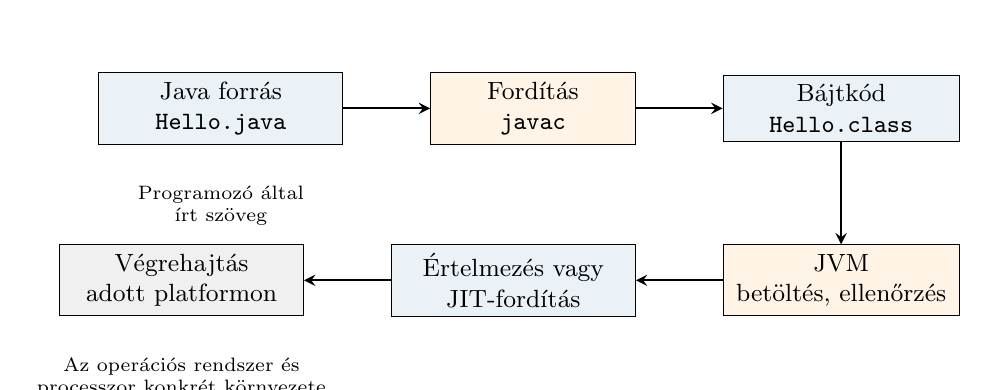
\begin{tikzpicture}[font=\small,node distance=11mm]
  \node[zvflowprocess, fill=lightaccent, minimum width=31mm] (source) {Java forrás\\\code{Hello.java}};
  \node[zvflowprocess, fill=warnbg, right=of source, minimum width=26mm] (javac) {Fordítás\\\code{javac}};
  \node[zvflowprocess, fill=lightaccent, right=of javac, minimum width=30mm] (class) {Bájtkód\\\code{Hello.class}};
  \node[zvflowprocess, fill=warnbg, below=13mm of class, minimum width=30mm] (jvm) {JVM\\betöltés, ellenőrzés};
  \node[zvflowprocess, fill=lightaccent, left=of jvm, minimum width=31mm] (jit) {Értelmezés vagy\\JIT-fordítás};
  \node[zvflowprocess, fill=black!6, left=of jit, minimum width=31mm] (native) {Végrehajtás\\adott platformon};

  \draw[arrow] (source) -- (javac);
  \draw[arrow] (javac) -- (class);
  \draw[arrow] (class) -- (jvm);
  \draw[arrow] (jvm) -- (jit);
  \draw[arrow] (jit) -- (native);

  \node[font=\scriptsize, align=center, below=4mm of source] {Programozó által\\írt szöveg};
  \node[font=\scriptsize, align=center, below=4mm of native] {Az operációs rendszer és\\processzor konkrét környezete};
\end{tikzpicture}
\caption{Java program fordításának és futtatásának szemléletes folyamata}
\label{fig:zv13_java_forditas_futtatas}
\end{figure}


\subsection{Fordítás és futtatás}

Egy egyszerű Java program fordítása és futtatása parancssorból:

\begin{itemize}
  \item fordítás: \code{javac Hello.java};
  \item eredmény: \code{Hello.class};
  \item futtatás: \code{java Hello}.
\end{itemize}

Ha a program csomagban van, akkor a könyvtárszerkezetnek és a futtatási osztálynévnek is illeszkednie kell a csomagnévhez. Például a \code{hu.example.zv13.HelloExam} teljes osztálynév azt jelzi, hogy az osztály a \code{hu.example.zv13} csomagban van.

\section{Egy Java program szerkezete}

\subsection{Fordítási egység}

A Java forrásfájl egy \textbf{fordítási egység}. Egy fordítási egység tipikus szerkezete:

\begin{enumerate}
  \item opcionális \code{package} utasítás;
  \item nulla vagy több \code{import} utasítás;
  \item osztály-, interfész-, enum- vagy rekorddefiníciók.
\end{enumerate}

A \code{package} utasításnak, ha van, a fájl elején kell állnia. Az \code{import} utasítások ezután következnek, majd a típusdefiníciók. Egy forrásfájlban több felső szintű típus is szerepelhet, de legfeljebb egy lehet \code{public}, és a \code{public} típus neve megegyezik a forrásfájl nevével.

\subsection{Csomagok}

A csomagok fő szerepei:

\begin{itemize}
  \item logikai egységekbe szervezik az osztályokat;
  \item névteret képeznek, ezért két külön csomagban lehet azonos nevű osztály;
  \item részt vesznek a hozzáférés-szabályozásban;
  \item segítik a nagyobb programok áttekinthető szervezését.
\end{itemize}

Egy osztály teljes neve a csomagnévből és az osztálynévből áll. Például:
\[
  \code{java.time.LocalDate}.
\]
A \code{java.time} itt csomagnév, a \code{LocalDate} pedig osztálynév.

A csomagnevek hierarchikusnak látszanak, de fontos, hogy az alcsomag nem valódi tartalmazást jelent. Ha importáljuk a \code{java.awt.*} csomagot, attól még a \code{java.awt.event} csomag osztályai nem importálódnak automatikusan.

\subsection{Importálás}

Az \code{import} nem másol be forráskódot, nem azonos a C nyelv \code{\#include} direktívájával. Az importálás csak azt teszi lehetővé, hogy egy osztályra a teljes név helyett rövid névvel hivatkozzunk.

Például:

\zvcode[language=Java,caption={Egyszerű Java fordítási egység csomaggal és importtal},label={lst:zv13_hello_package}]{src/code/zv13_hello_package.java}

A \code{java.lang} csomag automatikusan importálódik, ezért például a \code{String}, \code{System}, \code{Math} osztályokat külön import nélkül is használhatjuk.

\subsection{A main metódus}

A Java alkalmazás belépési pontja a \code{main} metódus. Klasszikus alakja:
\[
  \code{public static void main(String[] args)}.
\]

A részek jelentése:

\begin{itemize}
  \item \code{public}: a JVM kívülről eléri a metódust;
  \item \code{static}: a metódus osztályszintű, objektumpéldány létrehozása nélkül hívható;
  \item \code{void}: nincs visszatérési értéke;
  \item \code{String[] args}: a parancssori argumentumokat tartalmazó sztringtömb.
\end{itemize}

\section{Az objektumorientált programtervezés alapelvei}

\subsection{OOP szemlélet}

Az objektumorientált programtervezés szerint a program egymással együttműködő objektumok rendszere. Egy objektumnak van:

\begin{itemize}
  \item \textbf{azonossága}: megkülönböztethető más objektumoktól;
  \item \textbf{állapota}: az adattagok aktuális értékei;
  \item \textbf{viselkedése}: a rajta meghívható metódusok összessége.
\end{itemize}

Az osztály egy programozó által definiált típus, amely megadja az azonos szerkezetű és viselkedésű objektumok mintáját. Az objektum az osztály konkrét példánya.

\begin{center}
\begin{tabularx}{\textwidth}{L{30mm}X X}
\toprule
\textbf{Alapelv} & \textbf{Jelentése} & \textbf{Java-beli megvalósítási eszközök} \\
\midrule
Absztrakció & A lényeges tulajdonságok és műveletek kiemelése, a részletek elhagyása. & Osztályok, absztrakt osztályok, interfészek, metódusdeklarációk. \\
Egységbezárás & Az adatok és a rajtuk dolgozó műveletek egy egységbe, osztályba zárása. & Adattagok és metódusok ugyanabban az osztályban; objektumok állapottal és viselkedéssel. \\
Információrejtés & A belső reprezentáció és implementáció elrejtése a külvilág elől. & \code{private}, \code{protected}, \code{public}, csomagszintű láthatóság; getter/setter metódusok. \\
Öröklés & Új osztály létrehozása meglévő osztály specializálásával. & \code{extends}, metódusfelüldefiniálás, \code{super}; Java-ban osztályok között egyszeres öröklés van. \\
Kompozíció & Egy objektum más objektumokat tartalmaz, és azok szolgáltatásait használja. & Adattagként tárolt objektumreferenciák; gyakran rugalmasabb, mint az öröklés. \\
Polimorfizmus & Ugyanaz az üzenet/metódushívás többféle tényleges működést válthat ki. & Felüldefiniált metódusok dinamikus kötése, interfészek, absztrakt típusú referenciák. \\
\bottomrule
\end{tabularx}

\end{center}

\subsection{Egységbezárás és információrejtés}

Az \textbf{egységbezárás} azt jelenti, hogy az osztály egy egységbe zárja az adatokat és az ezekkel dolgozó műveleteket. Például egy \code{Circle} osztályban a sugár és a területszámítás metódusa ugyanahhoz a fogalomhoz tartozik.

Az \textbf{információrejtés} azt jelenti, hogy az objektum belső adatai kívülről nem érhetők el tetszőlegesen. A belső állapotot célszerű \code{private} adattagokkal védeni, és ellenőrzött metódusokon keresztül módosítani. Ez azért fontos, mert így az osztály megőrizheti saját invariánsait.

\subsection{Öröklés, kompozíció és polimorfizmus}

Az \textbf{öröklés} során egy osztály egy másik osztályból származik. Java-ban az osztályok között egyszeres öröklés van: egy osztály közvetlenül csak egy ősosztályból származhat. Interfészekből viszont többet is megvalósíthat.

A \textbf{kompozíció} azt jelenti, hogy egy objektum más objektumokat tartalmaz és azok szolgáltatásait használja. Például egy \code{Car} objektum tartalmazhat \code{Engine} objektumot. Gyakori tervezési elv, hogy ahol nem valódi ``az-egy'' kapcsolat van, ott az öröklés helyett a kompozíció tisztább megoldás.

A \textbf{polimorfizmus} lényege, hogy ugyanaz a metódushívás a futás közben hivatkozott objektum tényleges típusától függően más megvalósítást futtathat. Például egy \code{Shape} típusú referencia hivatkozhat \code{Circle} vagy \code{Rectangle} objektumra, és az \code{area()} hívás a tényleges objektumhoz tartozó területszámítást hajtja végre.

\section{Objektumok tárolása és élettartama}

\subsection{Referencia és objektum}

Java-ban az objektumokat nem közvetlenül változók tartalmazzák, hanem a változók objektumreferenciákat tárolnak. A referencia olyan érték, amelyen keresztül elérhető a heapen levő objektum. Emiatt két referencia mutathat ugyanarra az objektumra.

Példa:
\[
  \code{Student a = new Student("Anna");}
\]
Itt a \code{new Student("Anna")} létrehoz egy objektumot, az \code{a} változó pedig erre az objektumra hivatkozik.

\subsection{Stack, heap és statikus adatok}

A Java futásidejű memóriáját vizsgaszinten a következőképpen érdemes elképzelni:

\begin{itemize}
  \item a lokális változók és metódushívások adatai a hívási veremhez, vagyis stackhez kapcsolódnak;
  \item az objektumok tipikusan a heapen jönnek létre;
  \item a statikus tagok az osztályhoz kapcsolódnak, nem egy konkrét példányhoz;
  \item a metódusok kódja és az osztályok metaadatai a futtatókörnyezet osztálybetöltési mechanizmusához kapcsolódnak.
\end{itemize}

Fontos különbség: a lokális referencia változó megszűnhet a veremkeret eltűnésével, de az objektum csak akkor válik felszabadíthatóvá, ha már sehonnan sem érhető el.

\subsection{Példányosítás és konstruktor}

A példányosítás fő lépései:

\begin{enumerate}
  \item a \code{new} operátor memóriát foglal az objektumnak a heapen;
  \item az adattagok alapértelmezett értéket kapnak;
  \item lefut az inicializálás és a konstruktor;
  \item a létrejött objektum referenciája visszakerül a programhoz.
\end{enumerate}

\zvcode[language=Java,caption={Objektum létrehozása, használata és referencia elvesztése},label={lst:zv13_object_lifecycle}]{src/code/zv13_object_lifecycle.java}

A példában a \code{student = null;} nem közvetlenül törli az objektumot. Csak azt eredményezi, hogy ez a referencia már nem mutat rá. Ha más referencia sem éri el ugyanazt az objektumot, akkor az objektum szemétgyűjtésre alkalmassá válik.

\section{Szemétgyűjtő mechanizmus}

\subsection{A szemétgyűjtés célja}

A Java automatikus memóriakezelést használ. Ez azt jelenti, hogy a programozó nem hív explicit \code{free} vagy \code{delete} műveletet az objektumokra. A szemétgyűjtő, vagyis garbage collector feladata a már nem elérhető objektumok memóriájának felszabadítása.

Egy objektum akkor tekinthető élőnek, ha elérhető valamilyen \textbf{GC rootból}. Ilyen kiindulópont lehet például egy futó szál veremkeretében levő referencia vagy egy statikus referencia. Ha az objektumhoz nem vezet referenciaút, akkor szemétgyűjtésre jelölhető.

Ezt gráfosan is megfogalmazhatjuk. Legyenek az objektumok és referenciák egy irányított gráf csúcsai és élei. Egy objektum élő, ha van hozzá út valamely gyökérből:
\[
  \text{élő}(o)
  \quad\Longleftrightarrow\quad
  \exists r\in R: r \leadsto o,
\]
ahol $R$ a GC rootok halmaza.

\begin{figure}[htbp]
\centering
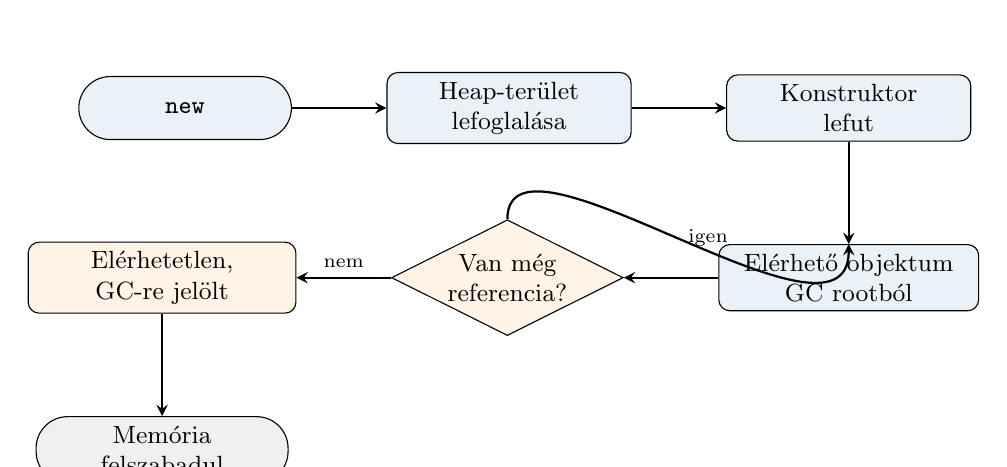
\begin{tikzpicture}[font=\small,node distance=12mm]
  \node[terminator, fill=lightaccent, minimum width=27mm] (start) {\code{new}};
  \node[flow, right=of start, minimum width=31mm] (alloc) {Heap-terület\\lefoglalása};
  \node[flow, right=of alloc, minimum width=31mm] (ctor) {Konstruktor\\lefut};
  \node[flow, below=13mm of ctor, minimum width=33mm] (reachable) {Elérhető objektum\\GC rootból};
  \node[pred, left=of reachable, minimum width=28mm] (lost) {Van még\\referencia?};
  \node[flow, left=of lost, minimum width=34mm, fill=warnbg] (eligible) {Elérhetetlen,\\GC-re jelölt};
  \node[terminator, below=13mm of eligible, fill=black!6, minimum width=32mm] (free) {Memória\\felszabadul};

  \draw[arrow] (start) -- (alloc);
  \draw[arrow] (alloc) -- (ctor);
  \draw[arrow] (ctor) -- (reachable);
  \draw[arrow] (reachable) -- (lost);
  \draw[arrow] (lost) -- node[above,font=\scriptsize]{nem} (eligible);
  \draw[arrow] (eligible) -- (free);
  \draw[arrow] (lost.north) .. controls +(0,14mm) and +(0,-16mm) .. node[right,font=\scriptsize]{igen} (reachable.north);
\end{tikzpicture}
\caption{Java objektum életútja a létrehozástól a szemétgyűjtésig}
\label{fig:zv13_objektum_elettartam_gc}
\end{figure}


\subsection{A szemétgyűjtés alaplépései}

Egy egyszerű szemlélet szerint a szemétgyűjtés lépései:

\begin{enumerate}
  \item a futtatókörnyezet megkeresi a gyökérreferenciákat;
  \item bejárja az innen elérhető objektumokat;
  \item az elérhető objektumokat élőként kezeli;
  \item a nem elérhető objektumok memóriája felszabadítható;
  \item szükség esetén a heap töredezettsége csökkenthető mozgatással vagy tömörítéssel.
\end{enumerate}

A konkrét JVM-ek többféle garbage collector algoritmust használhatnak. Vizsgaszinten a legfontosabb nem az algoritmus neve, hanem az elérhetőségi elv: nem az számít, hogy az objektumra valaha szükség volt-e, hanem az, hogy a program jelenlegi állapotából még elérhető-e.

\subsection{Mit nem garantál a szemétgyűjtés?}

A szemétgyűjtés nem jelenti azt, hogy az objektum memóriája azonnal felszabadul, amint elveszítjük az utolsó referenciát. A GC futását a JVM ütemezi, és nem determinisztikus, hogy pontosan mikor történik meg.

A szemétgyűjtés továbbá csak a memóriát kezeli automatikusan. Más erőforrásokat, például fájlokat, hálózati kapcsolatokat, adatbázis-kapcsolatokat továbbra is szabályosan le kell zárni. Java-ban erre célszerű a \code{try-with-resources} szerkezetet használni.

\begin{warningbox}
Gyakori félreértés, hogy a \code{System.gc()} biztosan azonnal felszabadítja a memóriát. Valójában ez legfeljebb kérés vagy jelzés a JVM felé, a szemétgyűjtés pontos idejét és módját nem szabad programlogikára építeni.
\end{warningbox}

\section{Kivételkezelés}

\subsection{A kivétel fogalma}

A \textbf{kivétel} a program futása közben bekövetkező rendellenes esemény objektumként való megjelenése. Kivétel keletkezhet például hibás indexeléskor, null referenciára való hivatkozáskor, fájlművelet sikertelenségekor vagy a programozó által kiadott \code{throw} utasítással.

Java-ban a kivételek osztályhierarchiába rendezett objektumok. A kivételobjektum információt hordoz a hiba típusáról és helyéről. A kivételkezelés célja, hogy a normál programlogika elkülönüljön a hibakezelő logikától.

\begin{center}
\begin{tabularx}{\textwidth}{L{29mm}L{48mm}X}
\toprule
\textbf{Elem} & \textbf{Feladat} & \textbf{Megjegyzés} \\
\midrule
\code{try} & A potenciálisan kivételt dobó normál kód helye. & A hibakezelő kódot nem ide, hanem a megfelelő \code{catch} ágba tesszük. \\
\code{catch} & A megadott típusú kivétel elkapása és kezelése. & Több \code{catch} esetén a specifikusabb kivételt kell előre írni. \\
\code{finally} & Mindenképpen lefutó lezáró blokk. & Erőforrás-felszabadításra használható, de Java-ban gyakran kiváltható \code{try-with-resources} szerkezettel. \\
\code{throw} & Kivétel kézi dobása. & Például hibás paraméter esetén saját kivétel dobható. \\
\code{throws} & Metódusfejlécben jelzi, hogy a metódus milyen ellenőrzött kivételt továbbíthat. & A hívónak kezelnie kell, vagy tovább kell jeleznie. \\
Ellenőrzött kivétel & Fordító által kikényszerített kezelés vagy továbbjelzés. & Példa: sok \code{IOException} jellegű hiba. \\
Nem ellenőrzött kivétel & \code{RuntimeException} vagy leszármazottja. & Általában programozási hibát vagy előfeltétel-sértést jelez, például \code{NullPointerException}. \\
\bottomrule
\end{tabularx}

\end{center}

\subsection{try, catch és finally}

A \code{try} blokkba kerül az a kód, amely kivételt dobhat. Ha kivétel keletkezik, a \code{try} blokk további utasításai nem futnak le, hanem a futtatókörnyezet megfelelő \code{catch} ágat keres. Az első olyan \code{catch} ág fut le, amelynek típusa képes kezelni a kivételt.

A \code{finally} blokk akkor is lefut, ha volt kivétel, és akkor is, ha nem. Ezért hagyományosan erőforrás-felszabadításra használták. Modern Java kódban fájlok és más lezárandó erőforrások esetén a \code{try-with-resources} gyakran jobb megoldás, mert automatikusan meghívja az erőforrás \code{close()} metódusát.

\subsection{throw és throws}

A \code{throw} utasítás egy konkrét kivételobjektumot dob:
\[
  \code{throw new IllegalArgumentException("hibás argumentum");}
\]

A \code{throws} a metódus fejlécében jelzi, hogy a metódus bizonyos kivételt nem kezel helyben, hanem továbbadja a hívónak. Ez különösen az ellenőrzött kivételeknél fontos, mert a fordító kikényszeríti a kezelésüket vagy továbbjelzésüket.

\zvcode[language=Java,caption={Kivétel továbbjelzése és try-with-resources használata},label={lst:zv13_exception_example}]{src/code/zv13_exception_example.java}

A példában az \code{IOException} ellenőrzött kivételként továbbadódhat a hívónak, ezért szerepel a metódus fejlécében a \code{throws IOException}. Az \code{IllegalArgumentException} ezzel szemben nem ellenőrzött kivétel, ezért nem kötelező feltüntetni a \code{throws} listában.

\subsection{Ellenőrzött és nem ellenőrzött kivételek}

Java-ban vizsgaszinten a következő felosztás fontos:

\begin{itemize}
  \item \textbf{ellenőrzött kivételek}: a fordító megköveteli, hogy kezeljük vagy \code{throws} segítségével továbbjelezzük őket;
  \item \textbf{nem ellenőrzött kivételek}: \code{RuntimeException} és leszármazottai, kezelésük nincs fordítási időben kikényszerítve;
  \item \textbf{súlyos hibák}: az \code{Error} típusú problémák többnyire a futtatókörnyezet súlyos állapotait jelzik, ezeket alkalmazáskódban általában nem kezeljük.
\end{itemize}

A jó kivételkezelés nem azt jelenti, hogy minden kivételt elnyelünk. A cél az, hogy ott kezeljük a hibát, ahol értelmes döntést tudunk hozni: javítani tudjuk a helyzetet, alternatív megoldást választunk, naplózunk, vagy érthető hibajelzést adunk.

\section{Gyakori félreértések}

\subsection{A bájtkód nem azonos a natív gépi kóddal}

A \code{javac} fordító \code{.class} bájtkódot készít. Ezt a JVM futtatja, értelmezi vagy JIT-fordítja. Ezért a Java fordítási modellje eltér a klasszikus C/C++ jellegű közvetlen natív fordítástól.

\subsection{Az import nem tölt be csomagot rekurzívan}

A \code{import java.awt.*;} csak a \code{java.awt} csomag közvetlen típusait teszi rövid néven elérhetővé. A \code{java.awt.event} külön csomag, ezért azt külön kell importálni, vagy teljes névvel kell hivatkozni rá.

\subsection{A referencia másolása nem objektummásolás}

Ha egy objektumreferenciát egy másik változóba másolunk, akkor nem jön létre új objektum. Csak két referencia fog ugyanarra az objektumra mutatni. Ezért az egyik referencián keresztüli állapotmódosítás a másikon keresztül is látható lesz.

\subsection{A szemétgyűjtő nem erőforráskezelő minden értelemben}

A GC a heapmemória felszabadításában segít, de nem helyettesíti a fájlok, adatbázis-kapcsolatok vagy hálózati kapcsolatok lezárását. Ezekre külön erőforrás-kezelési mintát kell használni, például \code{try-with-resources} szerkezetet.

\subsection{A kivételkezelés nem helyettesíti a feltételvizsgálatot}

A kivételek rendellenes helyzetek kezelésére valók. Nem célszerű normál vezérlési szerkezetként használni őket, mert rontják az olvashatóságot, és a hibás programlogikát elfedhetik.

\section{Tipikus vizsgakérdések és rövid válaszvázlatok}

\subsection{Mi a Java platformfüggetlenségének alapja?}

A Java forráskódból bájtkód készül, amelyet nem közvetlenül az operációs rendszer futtat, hanem a JVM. Ha egy platformon van megfelelő JVM, akkor ugyanaz a bájtkód elvileg futtatható rajta.

\subsection{Mi a különbség JDK, JRE és JVM között?}

A JDK fejlesztői csomag, amely fordítót is tartalmaz. A JRE futtatókörnyezet. A JVM a virtuális gép, amely a bájtkódot végrehajtja.

\subsection{Mi a fordítási egység Java-ban?}

Egy \code{.java} forrásfájl. Tartalmazhat \code{package} utasítást, importokat és típusdefiníciókat. Ha van \code{public} felső szintű osztály, a fájl neve ennek az osztálynak a nevéhez igazodik.

\subsection{Mire való a csomag?}

A csomag logikai szervezőegység és névtér. Segít elkerülni a névütközést, áttekinthetőbbé teszi a kódot, és szerepe van a hozzáférés-szabályozásban is.

\subsection{Melyek az OOP alapelvei?}

Absztrakció, egységbezárás, információrejtés, öröklés, kompozíció és polimorfizmus. Röviden: osztályokkal modellezünk, az adatokat és műveleteket egybe zárjuk, a belső részleteket elrejtjük, újrafelhasználunk és többalakú viselkedést teszünk lehetővé.

\subsection{Hol jönnek létre a Java objektumok?}

Tipikusan a heapen. A lokális változók referenciákat tárolhatnak a stackhez kapcsolódó veremkeretekben, de maga az objektum a heapen él, amíg elérhető.

\subsection{Mikor szabadítható fel egy objektum memóriája?}

Amikor már nem érhető el GC rootból, vagyis nincs hozzá élő referenciaút. Ekkor szemétgyűjtésre alkalmassá válik, de a tényleges felszabadítás idejét a JVM dönti el.

\subsection{Mi a kivételkezelés lényege?}

A rendellenes futási eseményeket kivételobjektumként kezeljük. A \code{try} blokkban fut a normál kód, a \code{catch} ágak kezelik a kivételeket, a \code{finally} pedig lezáró műveletekre szolgálhat.

\section{Összefoglalás vizsgára}

Rövid, vizsgán jól használható összefoglalás:

\begin{itemize}
  \item A Java fejlesztése a Sun Microsystems-nél indult, C/C++ jellegű szintaxist használ, de magasabb szintű és automatikus memóriakezelésű.
  \item A Java program \code{.java} forrásból \code{javac} segítségével \code{.class} bájtkódra fordul.
  \item A bájtkódot a JVM futtatja, ezért a Java platformfüggetlensége a virtuális géphez kapcsolódik.
  \item A JDK fejlesztéshez, a JRE futtatáshoz, a JVM pedig a bájtkód végrehajtásához szükséges.
  \item Egy Java fordítási egységben először \code{package}, majd \code{import}, végül típusdefiníciók állnak.
  \item A csomag névteret képez, hozzáférést szabályoz, és segíti a nagy programok szervezését.
  \item A \code{main} metódus klasszikus alakja: \code{public static void main(String[] args)}.
  \item Az OOP program együttműködő objektumok rendszere; az objektumnak állapota, viselkedése és azonossága van.
  \item Az OOP fő alapelvei: absztrakció, egységbezárás, információrejtés, öröklés, kompozíció, polimorfizmus.
  \item Java-ban az objektumokat referenciákon keresztül érjük el; a referencia másolása nem hoz létre új objektumot.
  \item Az objektumok tipikusan a heapen jönnek létre, a lokális referenciák a hívási veremhez kapcsolódnak.
  \item Az objektum akkor válik szemétgyűjtésre alkalmassá, ha már nincs elérhető referenciaút hozzá.
  \item A szemétgyűjtő a memóriát kezeli, de más erőforrásokat, például fájlokat, külön le kell zárni.
  \item A kivétel rendellenes futási eseményt leíró objektum.
  \item A kivételkezelés fő kulcsszavai: \code{try}, \code{catch}, \code{finally}, \code{throw}, \code{throws}.
  \item Az ellenőrzött kivételeket kezelni vagy továbbjelezni kell, a nem ellenőrzött kivételeknél ezt a fordító nem kényszeríti ki.
\end{itemize}

\end{document}
